\section{Powersupply}

\begin{enumerate}
  %\item Circuit design
  %\subitem In -> Out Voltage
  %\subitem Capacitors
  %\subitem Inductor
  \item PCB layout
  %\subitem Max current strength
  %\subsubitem > 2A -> Changed later
  \subitem Parasitic effects/interferences
\end{enumerate}

Because the speaker will be used with a Raspberry Pi or microcontroller, it should be compatible with an input voltage of $5V$. In order to provide the $24V$ needed by the amplifier circuit a boost converter is used.\p
The Class B Amplifier is designed to drive up to $100mA$. Aditionally the OpAmp itself and the circuit around it will need some current. Therefore the powersupply should provide at least $200mA$. Apart from this a higher switching frequency would help to reduce interferences at the speaker output.\p
%
Considering those requirements the LM2735 boost converter was chosen. Because the power usage of the ultrasonic transducers wasn't clear in the beginning of this project the powersupply provides up to $3A$ output current. The output voltage can be adjusted between $3V$ and $24V$.

\subsection{Circuit}

Figure \ref{fig:pcb:power_circuit} shows the circuit of the powersupply. The feedback was designed for using the equation given in the datasheet.
Note, \comp{R1} and \comp{R2} are switched compared to the circuit in the datasheet.
%
\begin{align}
  R_1 &= \left(\frac{V_{out}}{V_{ref}} - 1\right) \cdot R_2
  &\mathrm{with~} V_{ref} = 1.255V,~V_{out} = 24V
\end{align}
%
The dimensions of \comp{L1} as well as the capacity \comp{C7} and the diode \comp{D1} were taken from the examples in the datasheet.
%
\begin{figure}
  \centering
  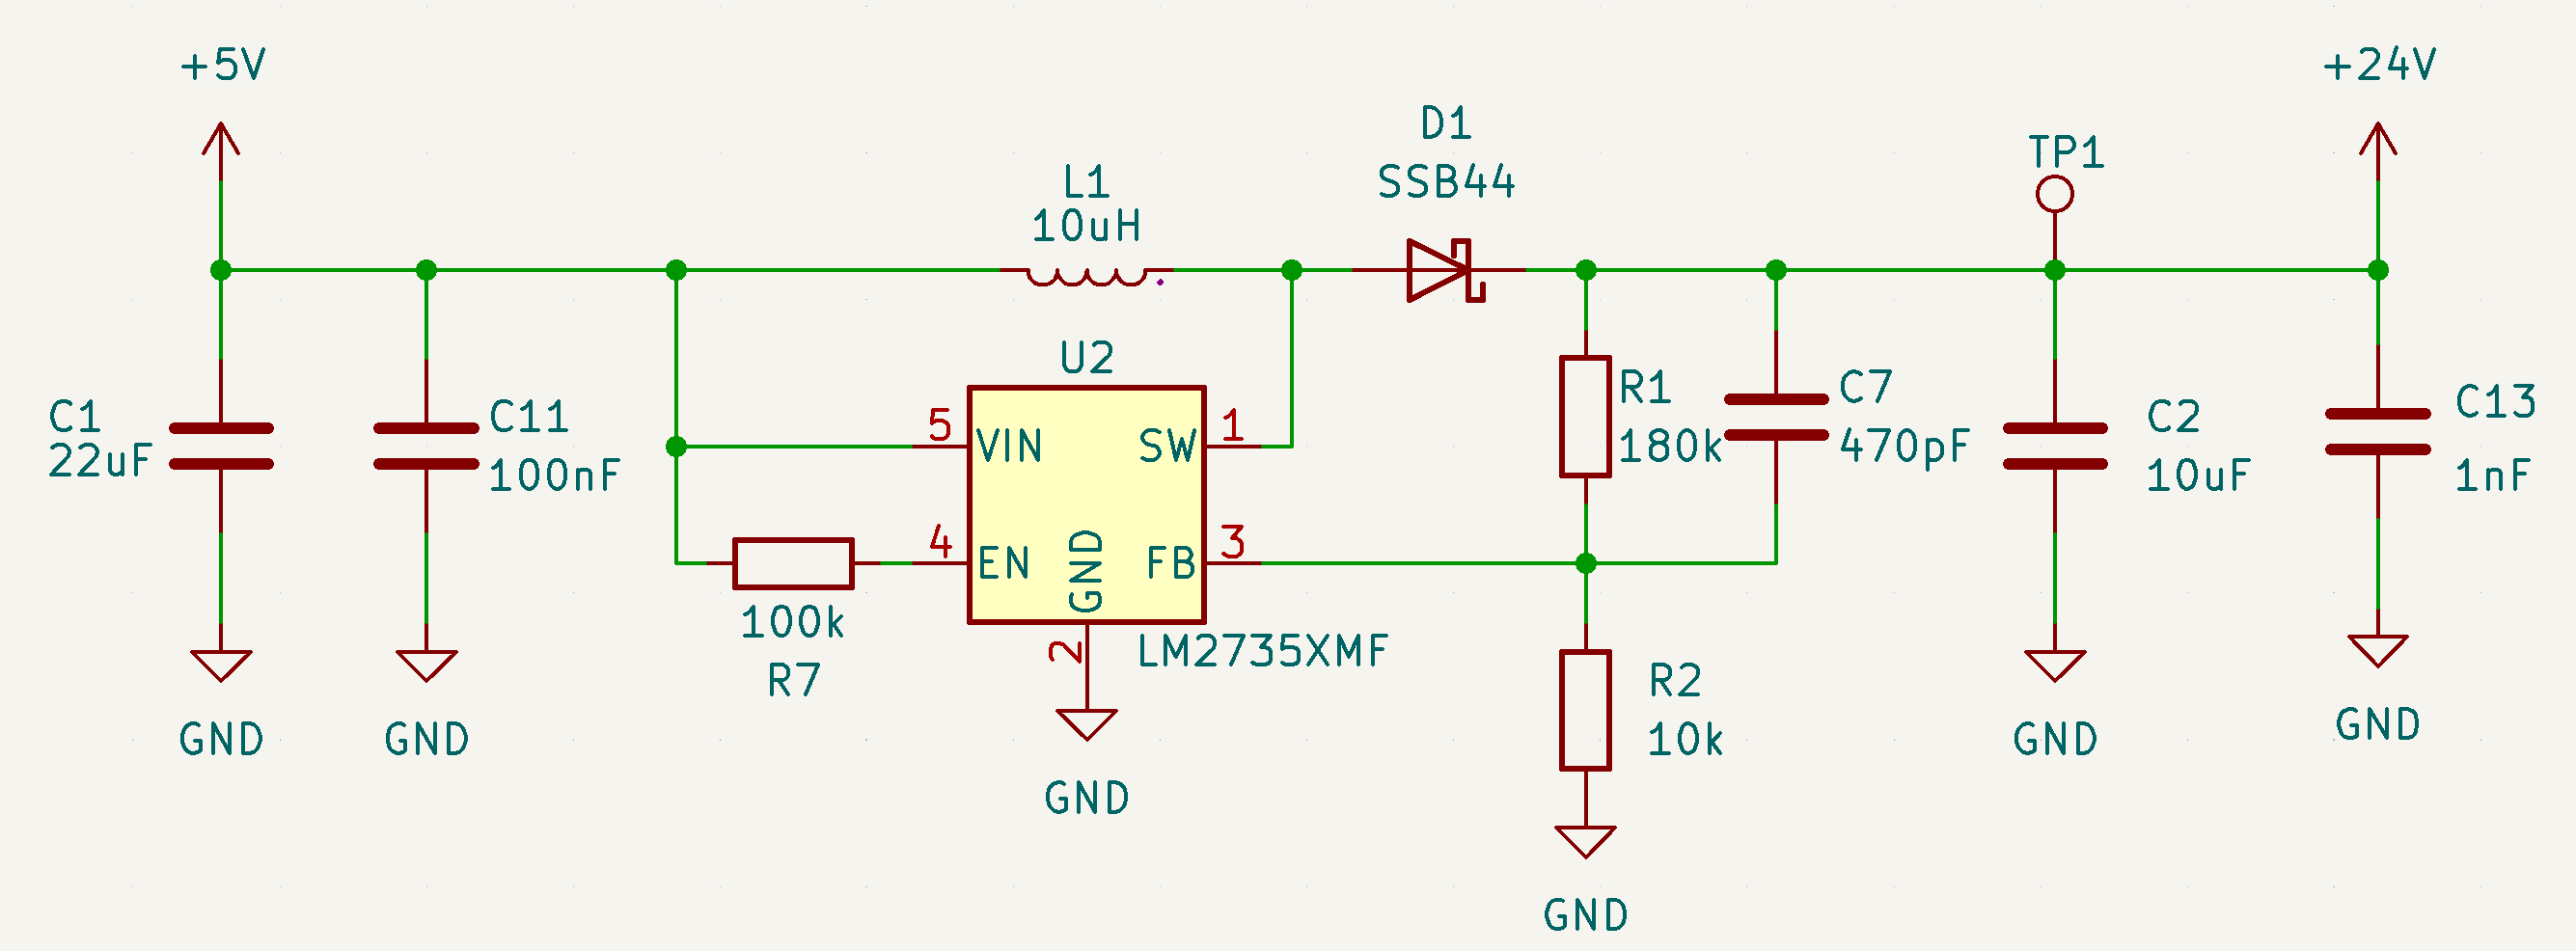
\includegraphics[width=\textwidth]{src/assets/pictures/circuit/powersupply_circuit.png}
  \caption{Powersupply circuit design}\label{fig:pcb:power_circuit}
\end{figure}